\documentclass[letterpaper]{article}
\usepackage[margin=1in]{geometry}
\usepackage[utf8]{inputenc}
\usepackage{textcomp}
\usepackage{amssymb}
\usepackage{natbib}
\usepackage{graphicx}
\usepackage{gensymb}
\usepackage{amsthm, amsmath, mathtools}
\usepackage[dvipsnames]{xcolor}
\usepackage{enumerate}
\usepackage{mdframed}
\usepackage[most]{tcolorbox}
\usepackage{csquotes}
% https://tex.stackexchange.com/questions/13506/how-to-continue-the-framed-text-box-on-multiple-pages

\tcbuselibrary{theorems}

\newcommand{\R}{\mathbb{R}}
\newcommand{\Z}{\mathbb{Z}}
\newcommand{\N}{\mathbb{N}}
\newcommand{\Q}{\mathbb{Q}}
\newcommand{\C}{\mathbb{C}}
\newcommand{\code}[1]{\texttt{#1}}
\newcommand{\mdiamond}{$\diamondsuit$}
\newcommand{\PowerSet}{\mathcal{P}}
\newcommand{\Mod}[1]{\ (\mathrm{mod}\ #1)}
\DeclareMathOperator{\lcm}{lcm}

%\newtheorem*{theorem}{Theorem}
%\newtheorem*{definition}{Definition}
%\newtheorem*{corollary}{Corollary}
%\newtheorem*{lemma}{Lemma}
\newtheorem*{proposition}{Proposition}


\newtcbtheorem[number within=section]{theorem}{Theorem}
{colback=green!5,colframe=green!35!black,fonttitle=\bfseries}{th}

\newtcbtheorem[number within=section]{definition}{Definition}
{colback=blue!5,colframe=blue!35!black,fonttitle=\bfseries}{def}

\newtcbtheorem[number within=section]{corollary}{Corollary}
{colback=yellow!5,colframe=yellow!35!black,fonttitle=\bfseries}{cor}

\newtcbtheorem[number within=section]{lemma}{Lemma}
{colback=red!5,colframe=red!35!black,fonttitle=\bfseries}{lem}

\newtcbtheorem[number within=section]{example}{Example}
{colback=white!5,colframe=white!35!black,fonttitle=\bfseries}{def}

\newtcbtheorem[number within=section]{note}{Important Note}{
        enhanced,
        sharp corners,
        attach boxed title to top left={
            xshift=-1mm,
            yshift=-5mm,
            yshifttext=-1mm
        },
        top=1.5em,
        colback=white,
        colframe=black,
        fonttitle=\bfseries,
        boxed title style={
            sharp corners,
            size=small,
            colback=red!75!black,
            colframe=red!75!black,
        } 
    }{impnote}
\usepackage[utf8]{inputenc}
\usepackage[english]{babel}
\usepackage{fancyhdr}
\usepackage[hidelinks]{hyperref}

\pagestyle{fancy}
\fancyhf{}
\rhead{MATH 155A}
\chead{Thursday, April 14, 2022}
\lhead{Lecture 6}
\rfoot{\thepage}

\setlength{\parindent}{0pt}

\begin{document}

\section{Moving to \texorpdfstring{$\R^3$}{Three-Dimensions}}
\subsection{Rigid \& Orientation-Preserving Transformations}

\subsubsection{Rigid, Orientation-Preserving Transformations in \texorpdfstring{$\R^2$}{Two-Dimensions}}
\begin{theorem}{}{}
    Let $A$ be a rigid, orientation-preserving map on $\R^2$. 
    \begin{enumerate}
        \item If $A(\mathbf{0}) = \mathbf{0}$, then $A$ is a rotation $R_{\theta}$ for some $\theta$. 
        \item If $A(\mathbf{u}) = \mathbf{u}$, then $A$ is a generalized rotation $R_{\theta}^{\mathbf{u}}$. 
        \item \emph{In general}, $A$ is either a translation $T_{\mathbf{u}}$ or a generalized rotation $R_{\theta}^{\mathbf{u}}$ for some $\mathbf{u}$ (and some $\theta$).
    \end{enumerate}
\end{theorem}

The proof for this theorem depends on this lemma:
\begin{lemma}{}{}
    Suppose $\mathbf{x} \neq \mathbf{y}$. Then, $A$ is uniquely determined by $\mathbf{u} = A(\mathbf{x})$ and $\mathbf{v} = A(\mathbf{y})$. 
\end{lemma}

\subsubsection{Euler's Theorem on Rotations in 3-Space}
\begin{theorem}{}{}
    Let $A: \R^3 \mapsto \R^3$ be a linear, orientation-preserving and rigid map. Then, $A$ is a rotation $R_{\theta, \mathbf{u}}$ for some $\theta$, $\mathbf{u}$ where $\mathbf{u} \neq 0$. 
\end{theorem}

\begin{lemma}{}{}
    Suppose $A(\mathbf{u}) = \mathbf{u}$ for some $\mathbf{u}$ such that $||\mathbf{u}|| = 1$. Then, $A$ is a rotation $R_{\theta, \mathbf{u}}$ for some $\theta$. 
\end{lemma}

What if $A$ is rigid, orientation-preserving, but $A(\mathbf{0}) \neq \mathbf{0}$? This is sometimes known as a glide rotation (or a screw motion).

\subsubsection{Finding the Center of Generalized Rotation}
Consider the following transformation:
\begin{center}
    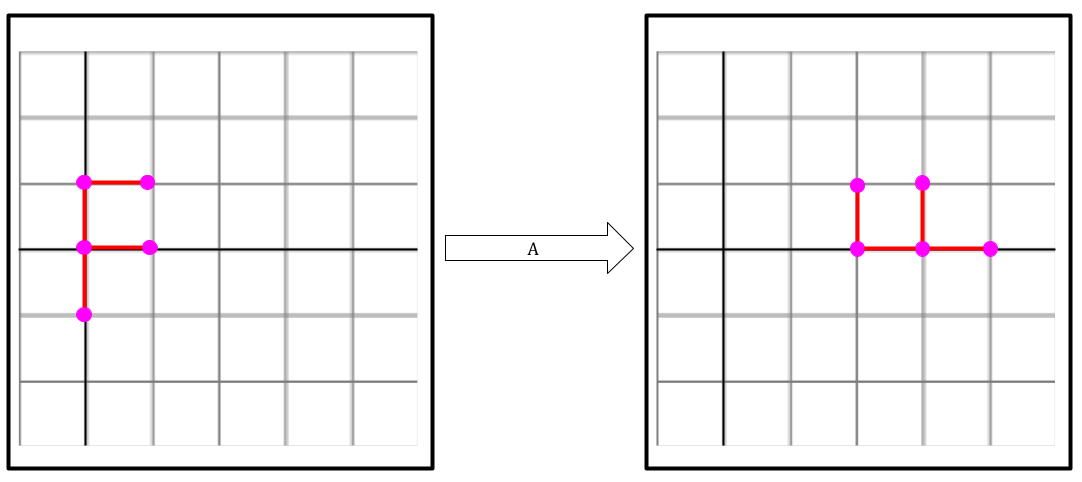
\includegraphics[scale=0.4]{../assets/gener.png}
\end{center}
Here, we have that $A(\mathbf{x}) = R_{90^{\circ}}(\mathbf{x}) + \begin{bmatrix}
    3 \\ 0
\end{bmatrix}$. In other words, $A = T_{\cyclic{3, 0}} \circ R_{90^{\circ}}$. Our goal is to express $A$ as a generalized rotation; that is, $A = R_{\theta}^{\mathbf{u}}$. It should be obvious that $\theta = 90^{\circ}$. Then, we need to find a $\mathbf{u}$ such that $A(\mathbf{u}) = \mathbf{u}$. 

\bigskip 

First, we want to choose a point $\mathbf{v}$ where $A(\mathbf{v}) \neq \mathbf{v}$. Let $\mathbf{w} = A(\mathbf{v})$.


\end{document}